\documentclass{article}

\usepackage{amsmath,amssymb,amsthm} % Advanced math typesetting
\usepackage[utf8]{inputenc} % Unicode support
\usepackage{hyperref} % Add a link to your document
\hypersetup{
    colorlinks,
    citecolor=blue,
    filecolor=black,
    linkcolor=blue,
    urlcolor=blue
}
\usepackage{tikz}
\usetikzlibrary{shapes.geometric}
\usetikzlibrary{arrows}
\usetikzlibrary{positioning}
\tikzstyle{ioblock} = [trapezium, trapezium left angle=70, trapezium right angle=110, minimum width = 3cm
, minimum height=1cm, text centered, draw=black, fill=orange!30]
\tikzstyle{processblock} = [rectangle, minimum width=3cm, minimum height=1cm, text centered, draw=black,
fill=orange!30]
\tikzstyle{decisionblock} = [diamond, minimum width=3cm, minimum height=1cm, text centered, draw=black,
fill = green!30]
\tikzstyle{arrow} = [thick,->,>=stealth]
\tikzstyle{startblock} = [rectangle, rounded corners, minimum width=3cm,
  minimum height=1cm,text centered, draw = black, fill=red!30]
\usepackage{graphicx} % Add pictures to your document
\usepackage{listings}
\usepackage{geometry}
 \geometry{
 a4paper,
 total={170mm,257mm},
 left=20mm,
 top=20mm,
 }
\usepackage{titling}
\usepackage{fancyhdr}
\fancypagestyle{plain}{%  the preset of fancyhdr 
    \fancyhf{} % clear all header and footer fields
    %\fancyfoot[R]{\includegraphics[width=2cm]{KULEUVEN_GENT_RGB_LOGO.png}}
    \fancyfoot[L]{\thedate}
    \fancyhead[L]{SPR200 Basic Cryptography}
    \fancyhead[R]{\theauthor}
}
\usepackage{cmbright}

\title{Lab-02: Describe Cryptographic Protocols \\ with Diagrams and Flowcharts}
\author{Avery Yong}
\date{January 18, 2025}
 

\makeatletter
\def\@maketitle{%
  \newpage
  \null
  \vskip 1em%
  \begin{center}%
  \let \footnote \thanks
    {\LARGE \@title \par}%
    \vskip 1em%
    %{\large \@date}%
  \end{center}%
  \par
  \vskip 1em}
\makeatother



\begin{document}

\maketitle

\noindent\begin{tabular}{@{}ll}
    Student Name & \theauthor\\
    Student \# & 059789115 \\
     Course Code &  SPR200\\
     Section Number & NAA \\
     Professor & Prof. Wei Huang 
\end{tabular}



\section{Practicing Flowchart}
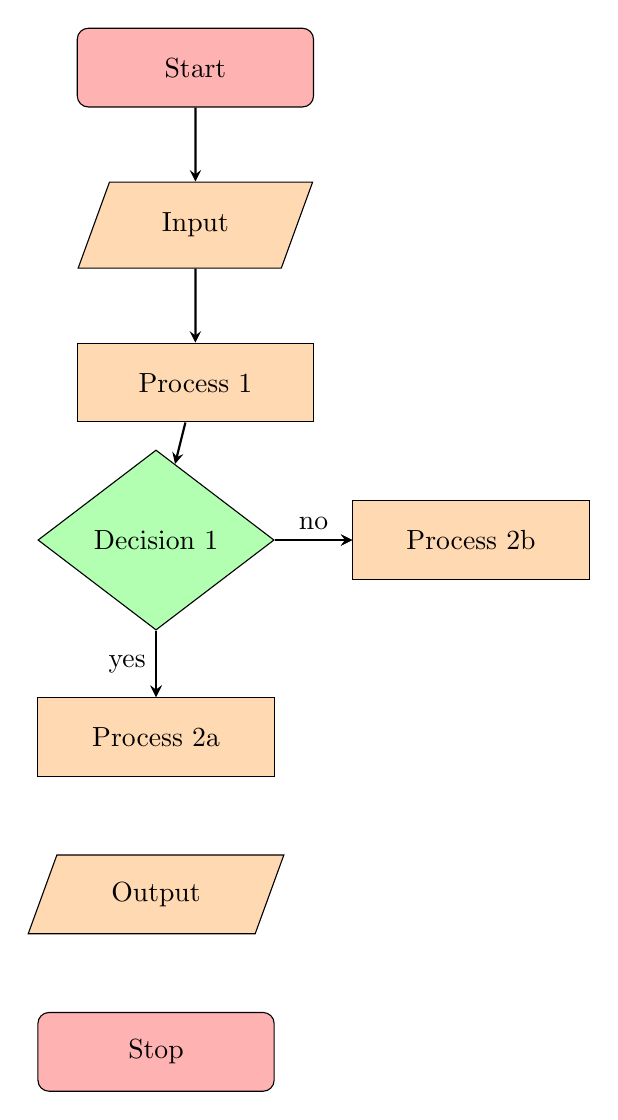
\begin{tikzpicture}[node distance=2cm]
  \node (start) [rectangle, rounded corners, minimum width=3cm,
  minimum height=1cm,text centered, draw = black, fill=red!30] {Start};
  \node (in1) [ioblock , below of = start] { Input };
  \node(pro1) [processblock,below of=in1] {Process 1};
  \node(dec1) [decisionblock,below of=pro1,xshift=-0.5cm] {Decision 1}; % yshift shifts down with negative
  % Then xshift negative shifts to the left (So remember it is like the cartesian plane)
  \node (pro2a) [processblock, below of=dec1, yshift = -0.5cm] {Process 2a};
  \node (pro2b) [processblock, right of=dec1, xshift = 2.0cm] {Process 2b};
  \node (out1) [ioblock, below of=pro2a] {Output};
  \node (stop) [startblock, below of=out1] {Stop};
  \draw [arrow] (start) -- (in1);
  \draw [arrow] (in1) -- (pro1);
  \draw [arrow] (pro1) -- (dec1);
  \draw [arrow] (dec1) -- (pro2a);
  \draw [arrow] (dec1) -- (pro2b); 
  \draw [arrow] (dec1) -- node[anchor=east] {yes} (pro2a);
  \draw [arrow] (dec1) -- node[anchor=south] {no} (pro2b);
\end{tikzpicture}


\section{Rainbow Attack Flowchart}

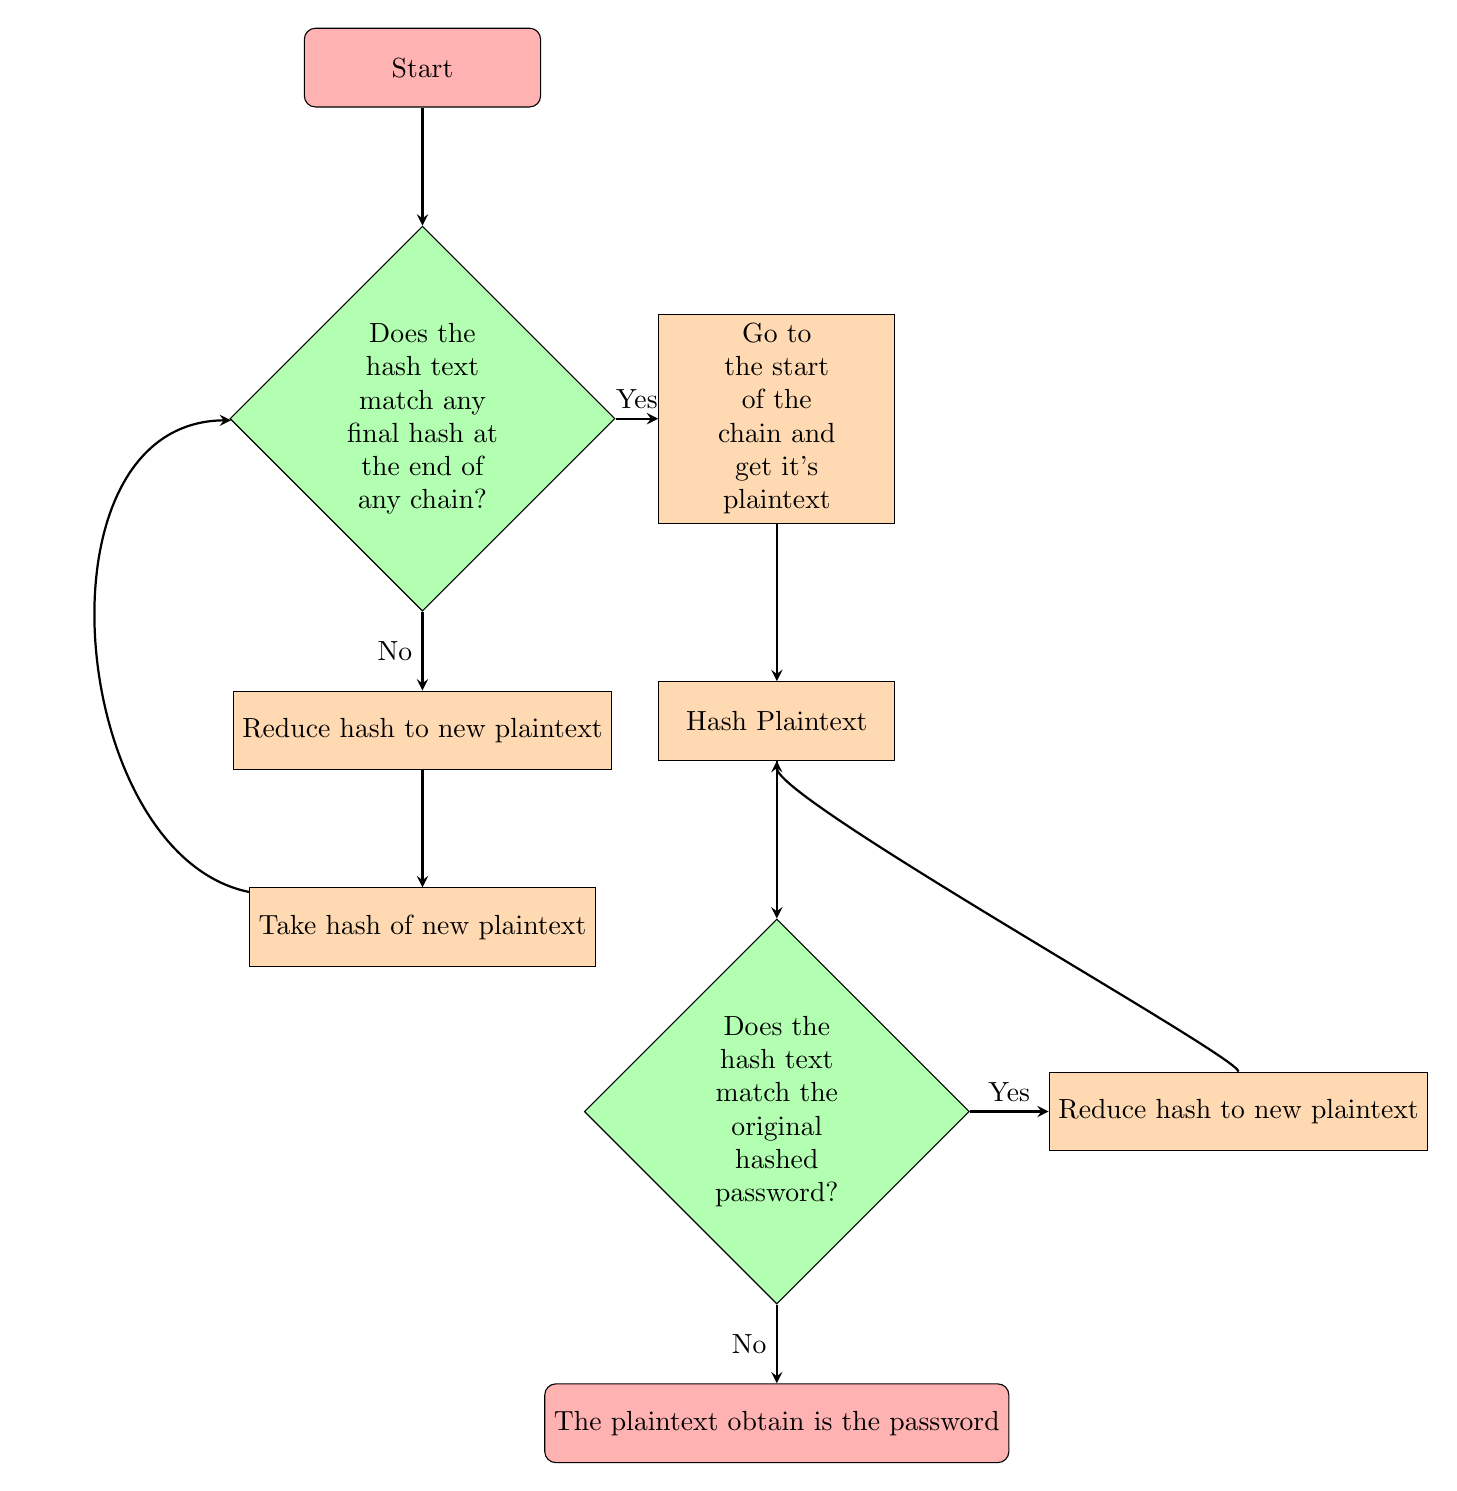
\begin{tikzpicture}[node distance=2cm] % what the heck this sucks lmao
  \node (start) [startblock] {Start};
  \node (d1) [decisionblock, below= 1.5cm of start, text width=20mm, align=center] {Does the hash text match any final hash at the end of any chain?};
  \node(p1) [processblock,below= 1cm of d1] {Reduce hash to new plaintext};
  \node (p1a) [ processblock, below of=p1, yshift = -0.5cm] {Take hash of new plaintext};
  \draw [arrow] (start) -- (d1);
  \draw [arrow] (d1) -- node[anchor=east]{No} (p1);
  \draw [arrow] (p1) -- (p1a);
  \draw [arrow] (p1a) .. controls (-4.5,-10) and (-5,-4.5) .. (d1);
  \node(p2) [processblock,right of=d1,xshift=2.5cm, text width=15mm, align=center] { Go to the start of the chain and get it's plaintext }; 
  \node(p2a) [processblock, below=of p2]{Hash Plaintext};
  \node(d2) [decisionblock, below=2cm of p2a, text width=20mm, align=center] {Does the hash text match the original hashed password?};
  \draw [arrow] (d1) -- node[anchor=south]{Yes} (p2);
  \draw [arrow] (p2) -- (p2a);
  \draw [arrow] (p2a) -- (d2);
  \node(p3a) [processblock, right=1cm of d2]{Reduce hash to new plaintext};
  \node(p3b) [startblock, below=1cm of d2] {The plaintext obtain is the password};
  \draw [arrow] (d2) -- node[anchor=east]{No} (p3b);
  \draw [arrow] (d2) -- node[anchor=south]{Yes}(p3a);
  \draw [arrow] (p3a)  .. controls +(up:7mm) and +(down:10mm) .. (p2a);
\end{tikzpicture}
\section{Hash Function Properties Diagram}

\begin {tikzpicture}
  \begin {scope}[ blend group = soft light ]
  \fill [red!30!black] (90:1.2) circle (2);
  \fill [yellow!30!] (210:1.2) circle (2);
  \fill [blue!30!white] (330:1.2) circle (2);
  \end {scope}
  \node at (90:2) {Preimage resistance};
  \node at (210:2) [text width=15mm,align=center] {Second preimage resistance};
  \node at (330:2) [text width=15mm,align=center]{Collision resistance};
  \node [font =\Large ] {Ideal};
\end {tikzpicture}

\section{Remote Coin-Flipping Protocol with One-Way Function}

\begin {center}
  \begin {tikzpicture}[>=latex]
  \coordinate (A) at (2,5);
  \coordinate (B) at (2,0);
  \coordinate (C) at (6,5);
  \coordinate (D) at (6,0);
  \draw[thick] (A)--(B) (C)--(D);
  \draw (A) node[above] {\Large Sean Feng};
  \draw (C) node[above] {\Large GF}; 
  \node(flip) [processblock] {I don't understand this still};

  \end{tikzpicture}
\end {center}


\end{document}
